\chapter{Prima Esercitazione}
%struttura di partenza
Il problema riguarda la risoluzione di una struttura iperstatica (riportata in figura \ref{fig:StrutturaDiPartenza}) soggetta a dei carichi tramite tre metodi: linea elastica, matriciale e FEM tramite il software Abaqus. 
\e stato richiesto inoltre il calcolo dello spostamento verticale nel nodo A e il confronto tra le sollecitazioni interne.
\begin{figure}[htb]
\centering
\begin{tikzpicture}
\scaling{5};
\point{a}{0}{0};
%\point{b}{.5}{0};
\point{c}{1}{0};
\point{d}{2}{.5};
\point{e}{2}{1};
\point{f}{1}{1};
\point{g}{1.12}{1}; %solo per il carrello
\point{h}{1.04}{0.025}; %solo per la cerniera
\point{i}{1.12}{1}; %solo per l'asta che non taglia il carrello
\beam{2}{a}{c}[0][1];
\beam{2}{c}{d}[1][1];
\beam{2}{d}{e}[1][1];
\beam{2}{e}{i}[1][1];
\beam{2}{f}{c}[1][1];
\support{3}{a}[-90]; %incastro % va in senso antiorario
\support{5}{f}[-90]; %molla
\support{2oowh}{g}[-90]; %senza il riempimento sotto
\hinge{1}{h}; %cerniera
\lineload{1}{i}{e}[1][1][.7]; 
\load{1}{d}[90][.8][-1];
\temperature{a}{c}{-.5}{.5}[.5][$+ \Delta T$][$- \Delta T$];
\dimensioning{1}{a}{c}{-1.5}[$l$];
\dimensioning{1}{c}{e}{-1.5}[$l$];
\dimensioning{2}{d}{e}{11.5}[$l/2$];
\dimensioning{2}{c}{d}{11.5}[$l/2$];
\notation{1}{e}{$q$}[above=1.4];
\notation{1}{d}{$F$}[below right];
\notation{1}{f}{$k$}[above left=.6];
\notation{1}{c}{$A$}[below right];
\end{tikzpicture}
\caption{Struttura di partenza}
\end{figure}%
\begin{table}[htb]
    \centering
    \caption[Effetti prodotti dai singoli carichi a varie intensità]{Effetti prodotti dei singoli carichi a varie intensità. Ogni riga indica l'azione che il carico crea nel caso tutti gli altri siano nulli nel nodo 2}
    \label{tab:confrontoSingoliCarichi}
    \begin{tabular}{l
                    S[table-format=1.5,
                      table-figures-exponent=2,
                      table-sign-mantissa,
                      table-sign-exponent]    
                    S[table-format=1.5,
                      table-figures-exponent=2,
                      table-sign-mantissa,
                      table-sign-exponent]
                    S[table-format=1.5,
                      table-figures-exponent=2,
                      table-sign-mantissa,
                      table-sign-exponent]}  
        \toprule
    	Azione & \multicolumn{1}{c}{$U_1$} & \multicolumn{1}{c}{$U_2$}& \multicolumn{1}{c}{$UR_3$}\\
    	& \multicolumn{1}{c}{\SI{}{\meter}} & \multicolumn{1}{c}{\SI{}{\meter}}& \multicolumn{1}{c}{\SI{}{\radian}}\\
	\midrule
	$\Delta T = \SI{40}{\degree}$ & 6.2052e-6   & -2.4687e-2  & -1.6458e-2\\
	$\Delta T = \SI{100}{\degree}$ & 1.5513e-5  &-6.1718e-2 & -4.1145e-2\\
	$F = \SI{600}{\newton}$ & -3.54432e-6 & 1.1858e-2  &  6.40955e-3\\
	$q = \SI{300}{\newton\per\meter}$ & -3.38322e-6 &  1.3459e-2 &  6.73009e-3\\
	\bottomrule
\end{tabular}
\end{table}

I valori di $q$, $F$, $k$ e $\Delta T$ sono stati assegnati in modo tale che gli effetti  tensionali di ciascuno di essi fosse confrontabile con quello degli altri. 
Dopo varie prove riportate in tabella \ref{tab:confrontoSingoliCarichi} si sono ottenuti i seguenti valori, con i quali si sono eseguiti tutti i successivi calcoli:
\begin{align*}
	q &= \SI{300}{\newton \per \metre}\\
	F &= \SI{600}{\newton}\\
	k &= \SI{22289.6}{\newton \per \metre}\\
	\Delta T &= \SI{40}{\celsius}
\end{align*}
La sezione delle travi in acciaio è stata scelta facendo attenzione ad avere una trave snella ovvero avendo una lunghezza pari a $10$ volte lo spessore medio e rispettando la verifica a presso-flessione in campo elastico 
\[
\frac{N}{A} + \frac{M}{W} < \SI{200}{\mega\pascal}
\]
portando ad avere, dopo varie iterazioni, dei tubi in acciaio a sezione quadrata con le seguenti caratteristiche:
\begin{center}
\begin{minipage}{6cm}
	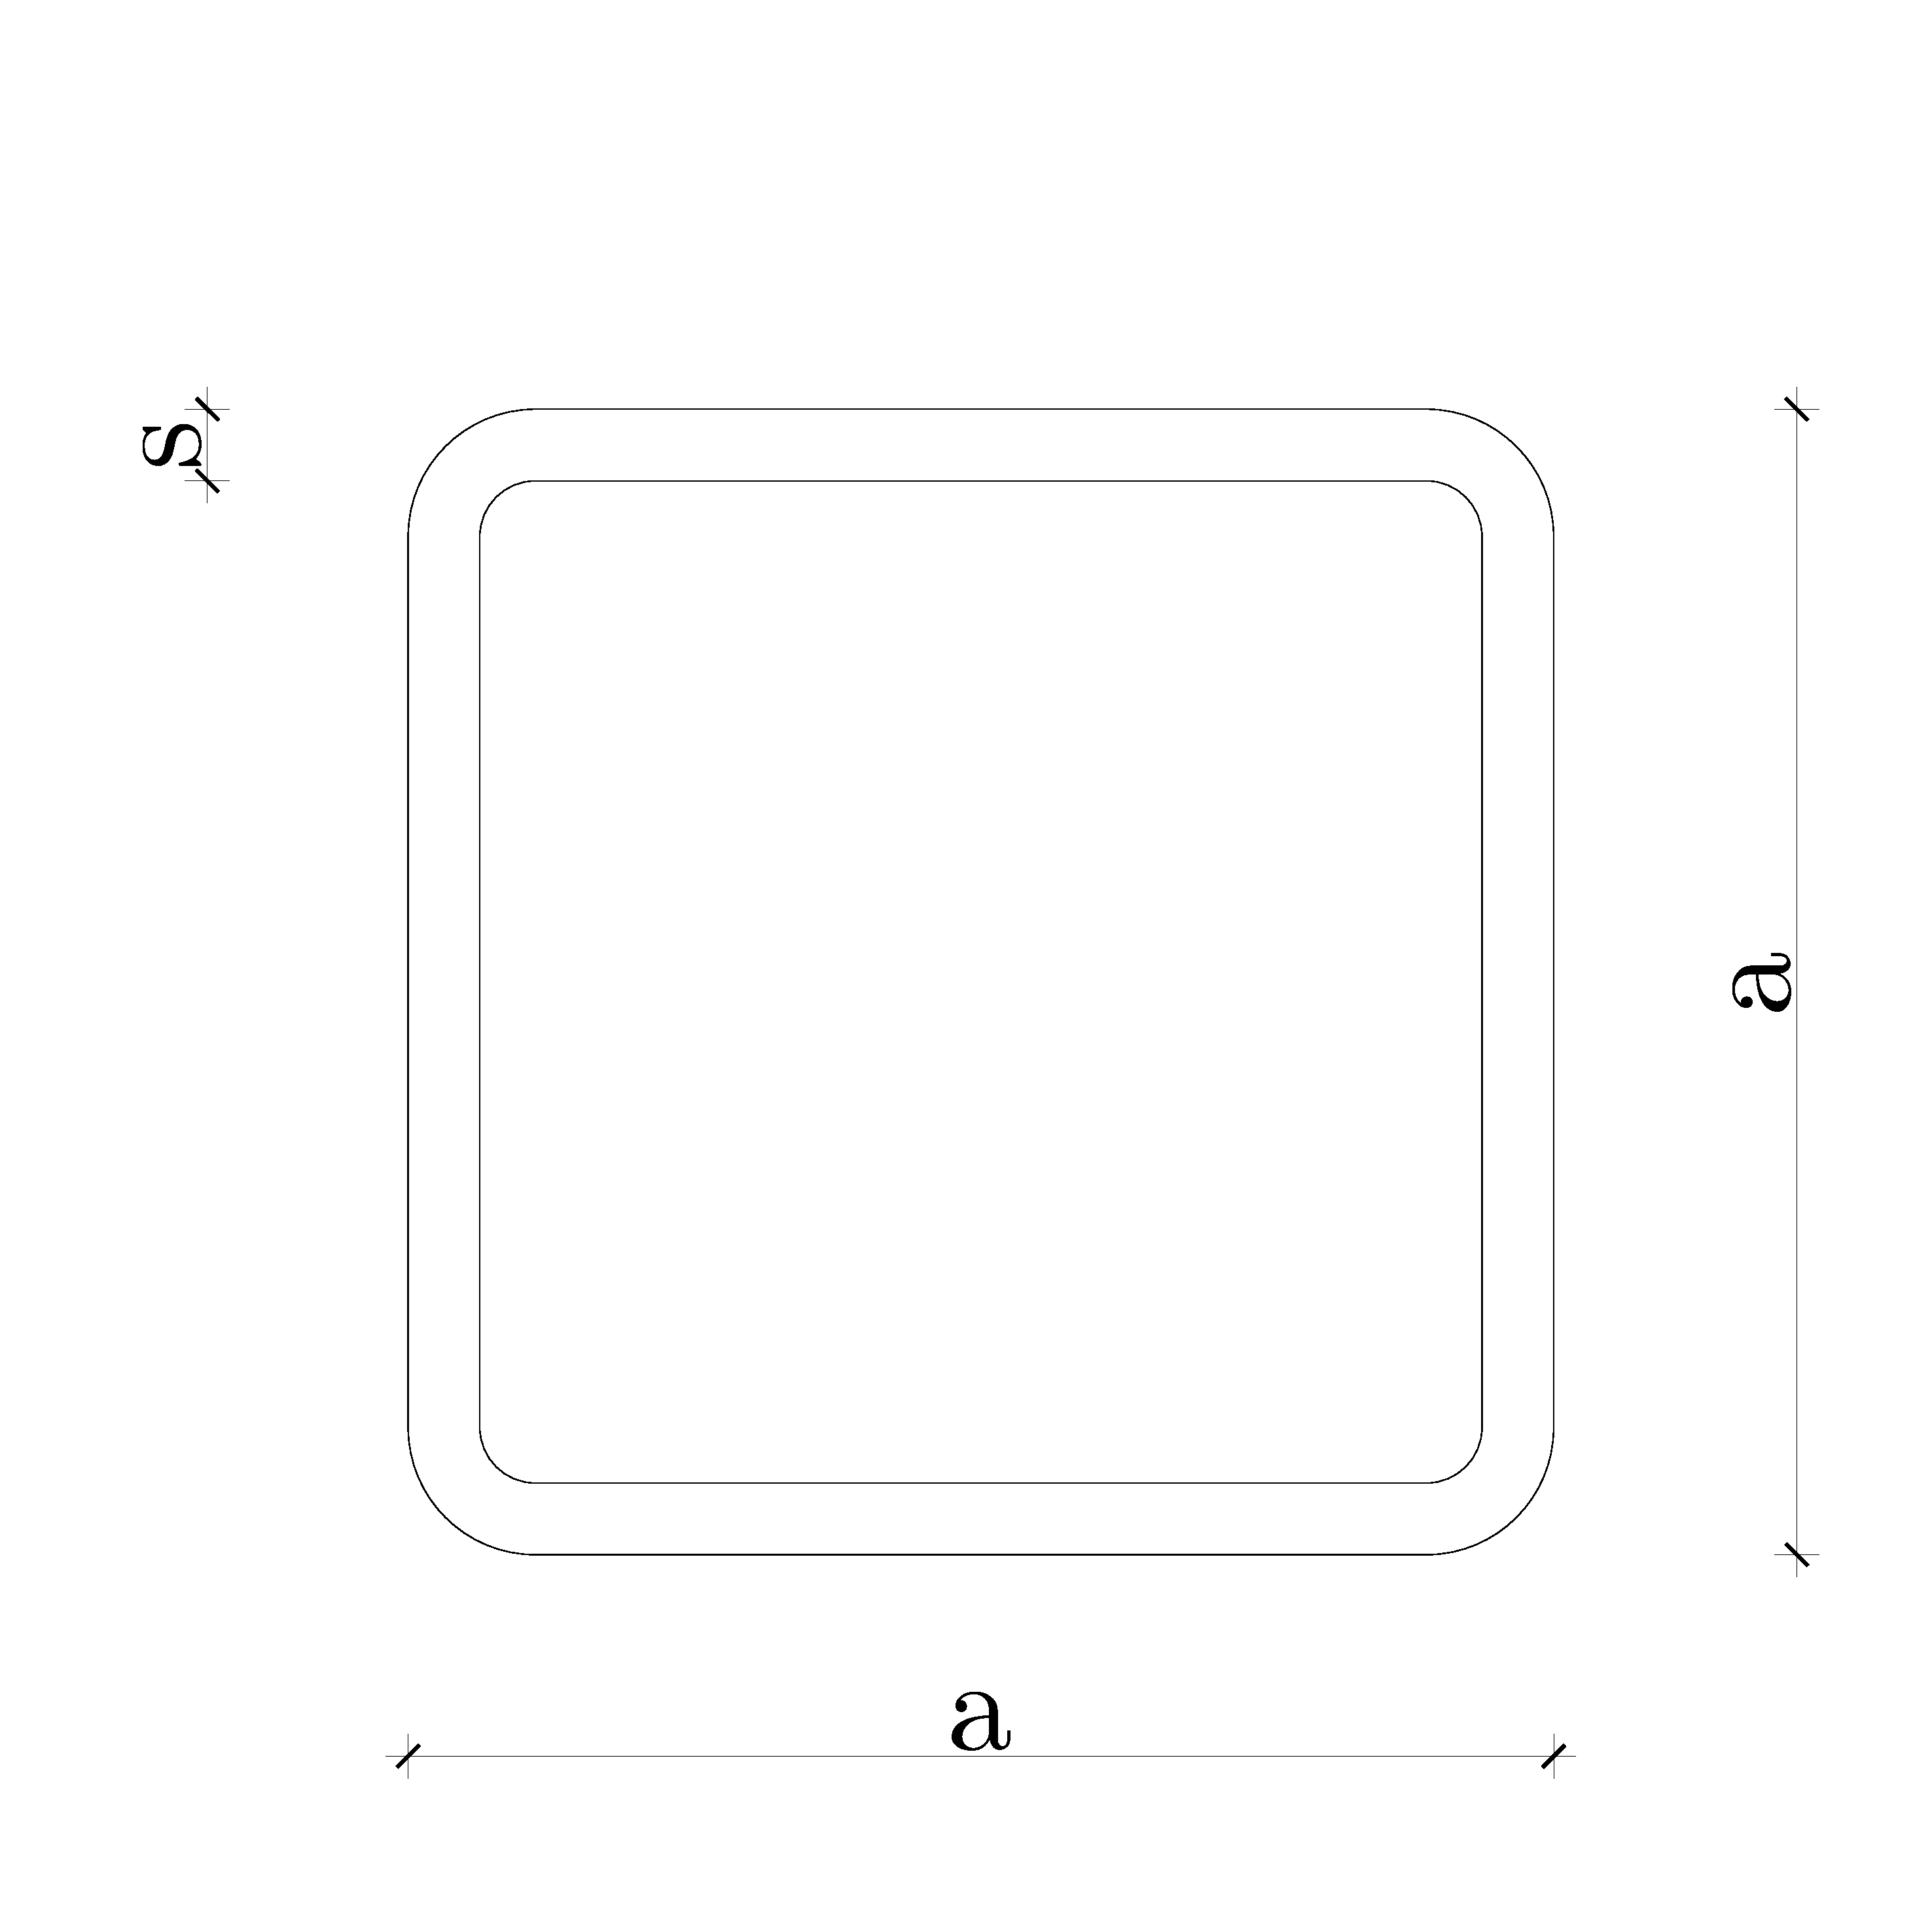
\includegraphics[width=60mm]{rel1/img1/tubi-quadri.pdf}
\end{minipage}
\begin{minipage}{6cm}
	\begin{align*}
		a &= \SI{100}{\milli\metre}\\
		s &= \SI{5}{\milli\metre}\\
		A &= \SI{19.00}{\centi\metre\squared}\\
		J_X = J_y &= \SI{286.58}{\centi\metre\tothe{4}}\\
		W_x = W_y &= \SI{57.32}{\centi\metre\cubed}
	\end{align*}
\end{minipage}
\end{center}
La verifica risulta pertanto verificata nelle due combinazioni tra sforzo normale e momento peggiori: 
\begin{align*}
    \sigma_1 &= \frac{N}{A} + \frac{M_{max}}{W} = \frac{\SI{96.07}{\newton}}{\SI{0.0019}{\metre\squared}} + \frac{\SI{7362}{\newton\metre}}{\SI{5.732e-5}{\metre\cubed}} = \SI{128}{\mega\pascal}< \SI{200}{\mega\pascal}\\
    \sigma_2 &= \frac{N_{max}}{A} + \frac{M}{W} = \frac{\SI{1610}{\newton}}{\SI{0.0019}{\metre\squared}} + \frac{\SI{2925}{\newton\metre}}{\SI{5.732e-5}{\metre\cubed}} =\SI{51.9}{\mega\pascal} < \SI{200}{\mega\pascal}
\end{align*}
%Struttura con i nomi ai punti
La figura \ref{fig:StrutturaConNomenclatura} a pagina \pageref{fig:StrutturaConNomenclatura} mostra la nomenclatura data ai nodi e alle aste. Il sistema di riferimento utilizzato varia in base al metodo utilizzato.

Si elencheranno ora le tre diverse tipologie di risoluzione del problema spiegando sinteticamente i passaggi effettuati. 
In figura \ref{fig:DiagrammiFinali} a pagina \pageref{fig:DiagrammiFinali} sono rappresentati i diagrammi delle sollecitazioni e la deformata della struttura.
Infine nel paragrafo \ref{cap:cap4} è presente un confronto dei risultati ottenuti con i diversi metodi.
\begin{figure}[htb]
\centering
\begin{tikzpicture}
\scaling{5};
\point{a}{0}{0};
%\point{b}{.5}{0};
\point{c}{1}{0};
\point{d}{2}{.5};
\point{e}{2}{1};
\point{f}{1}{1};
\beam{2}{a}{c}[0][1];
\beam{2}{c}{d}[1][1];
\beam{2}{d}{e}[1][1];
\beam{2}{e}{f}[1][1];
\beam{2}{f}{c}[1][1];
\dimensioning{1}{a}{c}{-1.5}[$l$];
\dimensioning{1}{c}{e}{-1.5}[$l$];
\dimensioning{2}{d}{e}{11.5}[$l/2$];
\dimensioning{2}{c}{d}{11.5}[$l/2$];
%disegno assi
%   \begin{scope}[color=red]
%       \load{1}{a}[180][1][-1];
%       \load{1}{a}[-90][1][-1];
%       \load{1}{c}[180][1][-1];
%       \load{1}{c}[-90][1][-1];
%       \load{1}{d}[180][1][-1];
%       \load{1}{d}[-90][1][-1];
%   \end{scope}
%nomi aste
\notation{4}{a}{c}[$1$];
\notation{4}{c}{d}[$5$];
\notation{4}{d}{e}[$4$];
\notation{4}{f}{e}[$3$];
\notation{4}{c}{f}[$2$];
%nomi punti
\notation{6}{a}{1};
\notation{6}{c}{2};
\notation{6}{f}{3};
\notation{6}{e}{4};
\notation{6}{d}{5};
\end{tikzpicture}
\caption{Nomenclatura dei nodi e delle aste utilizzata nei calcoli successivi. Per semplificazione il nodo $A$ è stato ribattezzato come nodo 2. Nel caso di Abaqus si hanno due nodi sovrapposti 30 e 31.}
\label{fig:StrutturaConNomenclatura}
\end{figure}
%-----
	%\section{Analisi tramite PLV}
\e stata degradata la molla bla bla bla
%Diagramma momenti delle strutture 0 e 1
%FILE NON PIù UTILIZZATO
\begin{figure}[htb]
\centering 
\begin{minipage}[b]{0.5\textwidth}
\begin{tikzpicture}
\scaling{3.5};
\point{a}{0}{0};
%\point{b}{.5}{0};
\point{c}{1}{0};
\point{d}{2}{.5};
\point{e}{2}{1};
\point{f}{1}{1};
\point{g}{1.17}{1}; %solo per il carrello
\point{h}{1.04}{0.025}; %solo per la cerniera
\point{i}{1.17}{1}; %solo per l'asta che non taglia il carrello
\beam{2}{a}{c}[0][1];
\beam{2}{c}{d}[1][1];
\beam{2}{d}{e}[1][1];
\beam{2}{e}{i}[1][1];
\beam{2}{f}{c}[1][1];
\support{3}{a}[-90]; % va in senso antiorario
\support{2oowh}{g}[-90]; %senza il riempimento sotto
\hinge{1}{h}; %cerniera
\lineload{1}{i}{e}[1][1][.5];
\load{1}{d}[90][.8][-1];
\notation{1}{e}{$q$}[above=1.4];
\notation{1}{d}{$F$}[below right];
\notation{1}{c}{$A$}[below right];
%diagramma momenti:
\internalforces{a}{c}{-.7}{-.3};
\internalforces{c}{f}{-.3}{0};
\internalforces{c}{d}{0}{.5};
\internalforces{d}{e}{.5}{.3};
\internalforces{e}{g}{.3}{.3};
\end{tikzpicture}
\end{minipage}%
\begin{minipage}[b]{1\textwidth}
\begin{tikzpicture}
\scaling{3.5};
\point{a}{0}{0};
%\point{b}{.5}{0};
\point{c}{1}{0};
\point{d}{2}{.5};
\point{e}{2}{1};
\point{f}{1}{1};
\point{g}{1.17}{1}; %solo per il carrello
\point{h}{1.04}{0.025}; %solo per la cerniera
\point{i}{1.17}{1}; %solo per l'asta che non taglia il carrello
\beam{2}{a}{c}[0][1];
\beam{2}{c}{d}[1][1];
\beam{2}{d}{e}[1][1];
\beam{2}{e}{i}[1][1];
\beam{2}{f}{c}[1][1];
\support{3}{a}[-90]; % va in senso antiorario
\support{2oowh}{g}[-90]; %senza il riempimento sotto
\hinge{1}{h}; %cerniera
\begin{scope}[color=blue]
	\load{1}{f}[180][1][.2];
	\notation{1}{f}{$x_1$}[above left=.2];
\end{scope}
%diagrammi momenti:
\internalforces{a}{c}{-.7}{-.7};
\internalforces{c}{f}{-.7}{0};
\end{tikzpicture}
\end{minipage}%
\caption{Diagramma dei momenti delle strutture (0) e (1)}
\end{figure}
%tabella equazioni:
\begin{table}[H]
\caption{Equazioni dei momenti delle strutture (0) e (1)}
\[
\begin{array}{cccc}
	\toprule
	\textbf{Asta}&\textbf{Lunghezza} & \textbf{Struttura (0)} & \textbf{Struttura (1)}\\
	\midrule
	1&l&\dfrac{7}{2}ql^2-\left(F+ql\right)z&l\\[2ex]
	2&l&\dfrac{7}{2}ql^2-(F+ql)l-\left(F+\dfrac{ql}{2}\right)z &l-z\\
	3&l&\dfrac{qz^2}{2}&0\\[2ex]
	4&\dfrac{l}{2}&\dfrac{ql^2}{2}+\left(\dfrac{ql}{2} + ql\right)z&0\\[2ex]
	5&\sqrt{\dfrac{5}{4}}l&\sqrt{\dfrac{5}{4}}Fz&0\\
	\bottomrule
\end{array}
\]
\end{table}
%Diagramma sforzo normale strutture 0 e 1
\begin{figure}[htb]
\centering 
\begin{minipage}[b]{0.5\textwidth}
\begin{tikzpicture}
\scaling{3.5};
\point{a}{0}{0};
%\point{b}{.5}{0};
\point{c}{1}{0};
\point{d}{2}{.5};
\point{e}{2}{1};
\point{f}{1}{1};
\point{g}{1.17}{1}; %solo per il carrello
\point{h}{1.04}{0.025}; %solo per la cerniera
\point{i}{1.17}{1}; %solo per l'asta che non taglia il carrello
\beam{2}{a}{c}[0][1];
\beam{2}{c}{d}[1][1];
\beam{2}{d}{e}[1][1];
\beam{2}{e}{i}[1][1];
\beam{2}{f}{c}[1][1];
\support{3}{a}[-90]; % va in senso antiorario
\support{2oowh}{g}[-90]; %senza il riempimento sotto
\hinge{1}{h}; %cerniera
\lineload{1}{i}{e}[1][1][.5];
\load{1}{d}[90][.8][-1];
\notation{1}{e}{$q$}[above=1.4];
\notation{1}{d}{$F$}[below right];
\notation{1}{c}{$A$}[below right];
%diagramma N struttura 0:
\internalforces{c}{d}{-.9}{-.9}[0][orange];
\internalforces{d}{e}{.6}{.6}[0][orange];
\internalforces{e}{g}{.3}{.3}[0][orange];
\end{tikzpicture}
\end{minipage}%
\begin{minipage}[b]{1\textwidth}
\begin{tikzpicture}
\scaling{3.5};
\point{a}{0}{0};
%\point{b}{.5}{0};
\point{c}{1}{0};
\point{d}{2}{.5};
\point{e}{2}{1};
\point{f}{1}{1};
\point{g}{1.17}{1}; %solo per il carrello
\point{h}{1.04}{0.025}; %solo per la cerniera
\point{i}{1.17}{1}; %solo per l'asta che non taglia il carrello
\beam{2}{a}{c}[0][1];
\beam{2}{c}{d}[1][1];
\beam{2}{d}{e}[1][1];
\beam{2}{e}{i}[1][1];
\beam{2}{f}{c}[1][1];
\support{3}{a}[-90]; % va in senso antiorario
\support{2oowh}{g}[-90]; %senza il riempimento sotto
\hinge{1}{h}; %cerniera
\begin{scope}[color=blue]
	\load{1}{f}[180][1][.2];
	\notation{1}{f}{$x_1$}[above left=.2];
\end{scope}
%diagrammi N struttura 1:
\internalforces{a}{c}{-.7}{-.7}[0][orange];
\end{tikzpicture}
\end{minipage}%
\caption{Diagramma degli sforzi normali delle strutture (0) e (1)}
\end{figure}
\begin{align*}
	\mathscr{L}_{int} &= \mathscr{L}_{ext}	\\
	\eta_{01}+x_1 \eta_{11} + \eta_T &= - \eta_m V_3 \\
	& \qquad \eta_{01}= \frac{1}{EI}\sum_{k}\int_L m_0 \cdot m_1\\
	& \qquad \eta_{11}= \frac{1}{EI}\sum_{k}\int_L m_1 \cdot m_1\\
	& \qquad \eta_T = \frac{2 \alpha \Delta T}{H}l^2 \\
	& \qquad \eta_m = \frac{1}{k_m} \left( F+\frac{ql}{2}\right)\\
	 \hookrightarrow \quad  x_1 &= \frac{15}{2}ql
\end{align*}
	\pagebreak
\section{Analisi tramite linea elastica}
Come già anticipato per calcolare la soluzione analitica è stato utilizzato il metodo della linea elastica tramite l'ausilio del programma Mathematica.
Dopo aver fissato un sistema di riferimento globale e dei sistemi di riferimento locali per ogni elemento, si è proceduto con la definizione delle equazioni differenziali. 

La prima equazione differenziale di quarto grado omogenea o non omogenea di ogni elemento definisce la deformazione a flessione, mentre la seconda equazione differenziale del secondo ordine omogenea definisce la deformazione assiale della trave.

{\footnotesize{
\begin{align*}
    EI\frac{d^4\,v_1(x)}{d\,x^4} = 0 &\qquad
    EA\frac{d^2\,u_1(x)}{d\,x^2} = 0 \\
    EI\frac{d^4\,v_2(x)}{d\,x^4} = 0 &\qquad
    EA\frac{d^2\,u_2(x)}{d\,x^2} = 0 \\
    EI\frac{d^4\,v_3(x)}{d\,x^4} = q &\qquad
    EA\frac{d^2\,u_3(x)}{d\,x^2} = 0 \\
    EI\frac{d^4\,v_4(x)}{d\,x^4} = 0 &\qquad
    EA\frac{d^2\,u_4(x)}{d\,x^2} = 0 \\
    EI\frac{d^4\,v_5(x)}{d\,x^4} = 0 &\qquad
    EA\frac{d^2\,u_5(x)}{d\,x^2} = 0 
\end{align*}}}
In totale perciò si hanno 10 equazioni differenziali per un totale di 30 costanti di integrazione da definire e quindi 30 condizioni al contorno per risolvere il sistema.
Nella tabella \ref{tab:EqContornoLineaElastica} sono state riportate per ogni nodo le equazioni di congruenza tra gli spostamenti e le equazioni di equilibrio per le sollecitazioni.
\begin{table}[htb]
\footnotesize
\caption{Elenco delle condizioni al contorno adottate nei nodi della struttura}
\label{tab:EqContornoLineaElastica}
\centering
\[
\begin{array}{ccc}
\toprule	
\text{Nodo} & \text{Equazioni di congruenza} & \text{Equazioni di equilibrio} \\\midrule
\multirow{3}{*}{1} & u_1(0)=0 & \\
 & v_1(0)=0 & \\
 & v_1^\prime(0)=0 & \\\midrule
\multirow{5}{*}{2} & u_1\left(L\right)=-u_5\left(\sqrt{\frac{5}{4}}L\right)\frac{2}{\sqrt{5}} - v_5\left(\sqrt{\frac{5}{4}}L\right)\frac{1}{\sqrt{5}} & M_1(L) - M_2(0) =0\\
 & v_1\left(L\right)=u_5\left(\sqrt{\frac{5}{4}}L\right)\frac{1}{\sqrt{5}} - v_5\left(\sqrt{\frac{5}{4}}L\right)\frac{2}{\sqrt{5}} & N_2(0) - T_1(L) + T_5\left(\sqrt{\frac{5}{4}}L\right)\frac{2}{\sqrt{5}} - N_5\left(\sqrt{\frac{5}{4}}L\right)\frac{1}{\sqrt{5}}=0\\
 & u_1(L) = v_2(0) & T_2(0) - N_1(L) + N_5\left(\sqrt{\frac{5}{4}}L\right)\frac{2}{\sqrt{5}} + N_5\left(\sqrt{\frac{5}{4}}L\right)\frac{1}{\sqrt{5}}=0\\
 & v_1(L) = -u_2(0) & M_5\left(\sqrt{\frac{5}{4}}L\right)=0\\
 & v_1^\prime(L) = v_2^\prime(0) & \\\midrule
\multirow{5}{*}{3} & v_2(L) = u_3(0) & M_2(L)=0\\
 & & N_2(L)=0 \\
 & & M_3(0)=0 \\
 & & T_3(0)=0 \\
 & & N_3(0) - T_2(L) = k\, v_2(L)\\\midrule
\multirow{3}{*}{4} & u_3(L) = -v_4(0) & N_3(0)+T_4\left(\sqrt{\frac{5}{4}}L\right)=0 \\
 & v_3(L) = u_4(0) & N_4(0)-T_3\left(\sqrt{\frac{5}{4}}L\right)=0 \\
 & v_3^\prime(L) = v_4^\prime(0) & M_3\left(\sqrt{\frac{5}{4}}L\right)-M_4(0)=0 \\\midrule
\multirow{3}{*}{5} & v_4(L/2) = u_5(0)\frac{2}{\sqrt{5}} + v_5(0)\frac{1}{\sqrt{5}} & M_4(L/2) - M_5(0)=0\\
 & u_4(L/2) = u_5(0)\frac{1}{\sqrt{5}} - v_5(0)\frac{2}{\sqrt{5}} & T_4(L/2)-T_5(0)\frac{1}{\sqrt{5}} - N_5(0)\frac{2}{\sqrt{5}}=0\\
 & v_4^\prime(L/2) = v_5^\prime(0) & N_4(L/2)+T_5(0)\frac{2}{\sqrt{5}}-N_5(0)\frac{1}{\sqrt{5}}-F=0\\
\bottomrule
\end{array}
\]
\end{table}

Si è quindi risolto il sistema di equazioni differenziali tramite l'ausilio di Mathematica, trovando le funzioni degli spostamenti al variare di $x$:

{\footnotesize{
\begin{align*}
     u_1(x) &= -2.4087\times10^{-7}x\\
     v_1(x) &= -0.000415408 x^3 + 0.00131629 x^2 \\
     u_2(x) &= -0.00063059\\
     v_2(x) &= -0.00026418 x^3 +0.00237762 x^2-0.00331828 x-7.2234\times10^{-7}\\
     u_3(x) &= 2.63158 \times10^{-6}x +0.00431015\\
     v_3(x) &= 0.0000207704 x^4 -00734869x + 0.0379719\\
     u_4(x) &= -2.25564\times10^{-6} x+0.0176082\\
     v_4(x) &= 0.000290786 x^3+0.0011216 x^2-0.00510549 x-0.00431804\\
     u_5(x) &= -4.03501\times10^{-6} x+0.000296188\\
     v_5(x) &= -0.000241509 x^3+0.00243014 x^2 +0.000222117 x-0.0195347\\
\end{align*}}}
A cui poi applicando le formule di legame tra gli sforzi e sostituendo i valori di $x$, si è pervenuti ai valori di spostamento nel nodo richiesto ed ai valori di sforzo per il primo nodo. 
\begin{align*}
    M(x) &= -EI \left[v^{\prime\prime}(x) + \chi_{th}\right] \\
    T(x) &= M^\prime(x) \\
    N(x) &= EA \, u^\prime (x)
\end{align*}
\begin{align*}
    u_2 &= \SI{-7.22e-7}{\meter}\\
    v_2 &= \SI{6.31e-4}{\meter}\\
    M_1 &= \SI{-7.362e3}{\newton\meter}\\
    T_1 &= \SI{1.500e3}{\newton}\\
    N_1 &= \SI{-96.07}{\newton}\\
\end{align*}


    \section{Analisi tramite calcolo matriciale}
Come prima operazione è stato definito il vettore degli spostamenti:
\[
\overline{u}^T = \left[u_1,v_1,\varphi_1,u_2,v_2,\varphi_2,\varphi_2^{EF5},u_3,v_3^{EF2},v_3^{EF3},\varphi_3^{EF2},\varphi_3^{EF3},u_4,v_4,\varphi_4,u_5,v_5,\varphi_5 \right]
\]
Si sono quindi definite le matrici di assemblaggio e di rotazione per ciascun elemento.
%
%Matrici di assemblaggio
%
\begin{align*}
\mathbf{A_1} &=
{\arraycolsep=1pt\medmuskip=0.8mu\footnotesize
\left[
\begin{array}{cccccccccccccccccc}
 1 & 0 & 0 & 0 & 0 & 0 & 0 & 0 & 0 & 0 & 0 & 0 & 0 & 0 & 0 & 0 & 0 & 0 \\
 0 & 1 & 0 & 0 & 0 & 0 & 0 & 0 & 0 & 0 & 0 & 0 & 0 & 0 & 0 & 0 & 0 & 0 \\
 0 & 0 & 1 & 0 & 0 & 0 & 0 & 0 & 0 & 0 & 0 & 0 & 0 & 0 & 0 & 0 & 0 & 0 \\
 0 & 0 & 0 & 1 & 0 & 0 & 0 & 0 & 0 & 0 & 0 & 0 & 0 & 0 & 0 & 0 & 0 & 0 \\
 0 & 0 & 0 & 0 & 1 & 0 & 0 & 0 & 0 & 0 & 0 & 0 & 0 & 0 & 0 & 0 & 0 & 0 \\
 0 & 0 & 0 & 0 & 0 & 1 & 0 & 0 & 0 & 0 & 0 & 0 & 0 & 0 & 0 & 0 & 0 & 0 \\
 \end{array}
 \right]
 }
\qquad
 \mathbf{A_2} =
{\arraycolsep=1pt\medmuskip=0.8mu\footnotesize
\left[
\begin{array}{cccccccccccccccccc}
 0 & 0 & 0 & 1 & 0 & 0 & 0 & 0 & 0 & 0 & 0 & 0 & 0 & 0 & 0 & 0 & 0 & 0 \\
 0 & 0 & 0 & 0 & 1 & 0 & 0 & 0 & 0 & 0 & 0 & 0 & 0 & 0 & 0 & 0 & 0 & 0 \\
 0 & 0 & 0 & 0 & 0 & 1 & 0 & 0 & 0 & 0 & 0 & 0 & 0 & 0 & 0 & 0 & 0 & 0 \\
 0 & 0 & 0 & 0 & 0 & 0 & 0 & 1 & 0 & 0 & 0 & 0 & 0 & 0 & 0 & 0 & 0 & 0 \\
 0 & 0 & 0 & 0 & 0 & 0 & 0 & 0 & 1 & 0 & 0 & 0 & 0 & 0 & 0 & 0 & 0 & 0 \\
 0 & 0 & 0 & 0 & 0 & 0 & 0 & 0 & 0 & 0 & 1 & 0 & 0 & 0 & 0 & 0 & 0 & 0 \\
 \end{array}
 \right]
 }
 \\
 \mathbf{A_3} &=
{\arraycolsep=1pt\medmuskip=0.8mu\footnotesize
\left[
\begin{array}{cccccccccccccccccc}
 0 & 0 & 0 & 0 & 0 & 0 & 0 & 1 & 0 & 0 & 0 & 0 & 0 & 0 & 0 & 0 & 0 & 0 \\
 0 & 0 & 0 & 0 & 0 & 0 & 0 & 0 & 0 & 1 & 0 & 0 & 0 & 0 & 0 & 0 & 0 & 0 \\
 0 & 0 & 0 & 0 & 0 & 0 & 0 & 0 & 0 & 0 & 0 & 1 & 0 & 0 & 0 & 0 & 0 & 0 \\
 0 & 0 & 0 & 0 & 0 & 0 & 0 & 0 & 0 & 0 & 0 & 0 & 1 & 0 & 0 & 0 & 0 & 0 \\
 0 & 0 & 0 & 0 & 0 & 0 & 0 & 0 & 0 & 0 & 0 & 0 & 0 & 1 & 0 & 0 & 0 & 0 \\
 0 & 0 & 0 & 0 & 0 & 0 & 0 & 0 & 0 & 0 & 0 & 0 & 0 & 0 & 1 & 0 & 0 & 0 \\
 \end{array}
 \right]
 } 
 \qquad
 \mathbf{A_4} =
{\arraycolsep=1pt\medmuskip=0.8mu\footnotesize
\left[
\begin{array}{cccccccccccccccccc}
 0 & 0 & 0 & 0 & 0 & 0 & 0 & 0 & 0 & 0 & 0 & 0 & 1 & 0 & 0 & 0 & 0 & 0 \\
 0 & 0 & 0 & 0 & 0 & 0 & 0 & 0 & 0 & 0 & 0 & 0 & 0 & 1 & 0 & 0 & 0 & 0 \\
 0 & 0 & 0 & 0 & 0 & 0 & 0 & 0 & 0 & 0 & 0 & 0 & 0 & 0 & 1 & 0 & 0 & 0 \\
 0 & 0 & 0 & 0 & 0 & 0 & 0 & 0 & 0 & 0 & 0 & 0 & 0 & 0 & 0 & 1 & 0 & 0 \\
 0 & 0 & 0 & 0 & 0 & 0 & 0 & 0 & 0 & 0 & 0 & 0 & 0 & 0 & 0 & 0 & 1 & 0 \\
 0 & 0 & 0 & 0 & 0 & 0 & 0 & 0 & 0 & 0 & 0 & 0 & 0 & 0 & 0 & 0 & 0 & 1 \\
 \end{array}
 \right]
 }
\\
 \mathbf{A_5} &=
{\arraycolsep=1pt\medmuskip=0.8mu\footnotesize
\left[
\begin{array}{cccccccccccccccccc}
 0 & 0 & 0 & 0 & 0 & 0 & 0 & 0 & 0 & 0 & 0 & 0 & 0 & 0 & 0 & 1 & 0 & 0 \\
 0 & 0 & 0 & 0 & 0 & 0 & 0 & 0 & 0 & 0 & 0 & 0 & 0 & 0 & 0 & 0 & 1 & 0 \\
 0 & 0 & 0 & 0 & 0 & 0 & 0 & 0 & 0 & 0 & 0 & 0 & 0 & 0 & 0 & 0 & 0 & 1 \\
 0 & 0 & 0 & 1 & 0 & 0 & 0 & 0 & 0 & 0 & 0 & 0 & 0 & 0 & 0 & 0 & 0 & 0 \\
 0 & 0 & 0 & 0 & 1 & 0 & 0 & 0 & 0 & 0 & 0 & 0 & 0 & 0 & 0 & 0 & 0 & 0 \\
 0 & 0 & 0 & 0 & 0 & 0 & 1 & 0 & 0 & 0 & 0 & 0 & 0 & 0 & 0 & 0 & 0 & 0 \\
 \end{array}
 \right]
 }
 \end{align*}%
%
%Matrici di rotazione
%
\begin{align*}
\mathbf{T_1}=\mathbf{T(0)} &=
{\arraycolsep=3pt\medmuskip=0.8mu\footnotesize
\left[
\begin{array}{cccccc}
 1 & 0 & 0 & 0 & 0 & 0 \\
 0 & 1 & 0 & 0 & 0 & 0 \\
 0 & 0 & 1 & 0 & 0 & 0 \\
 0 & 0 & 0 & 1 & 0 & 0 \\
 0 & 0 & 0 & 0 & 1 & 0 \\
 0 & 0 & 0 & 0 & 0 & 1 \\
\end{array}
 \right]
 }
\qquad
\mathbf{T_2}=\mathbf{T(-\pi/2)} =
{\arraycolsep=3pt\medmuskip=0.8mu\footnotesize
\left[
\begin{array}{cccccc}
 0 & -1 & 0 & 0 & 0 & 0 \\
 1 & 0 & 0 & 0 & 0 & 0 \\
 0 & 0 & 1 & 0 & 0 & 0 \\
 0 & 0 & 0 & 0 & -1 & 0 \\
 0 & 0 & 0 & 1 & 0 & 0 \\
 0 & 0 & 0 & 0 & 0 & 1 \\
\end{array}
 \right]
 }
 \\
 \mathbf{T_3}=\mathbf{T(0)} &=
{\arraycolsep=3pt\medmuskip=0.8mu\footnotesize
\left[
\begin{array}{cccccc}
 1 & 0 & 0 & 0 & 0 & 0 \\
 0 & 1 & 0 & 0 & 0 & 0 \\
 0 & 0 & 1 & 0 & 0 & 0 \\
 0 & 0 & 0 & 1 & 0 & 0 \\
 0 & 0 & 0 & 0 & 1 & 0 \\
 0 & 0 & 0 & 0 & 0 & 1 \\
\end{array}
 \right]
 } 
 \qquad
 \mathbf{T_4}=\mathbf{T(\pi/2)} =
{\arraycolsep=3pt\medmuskip=0.8mu\footnotesize
\left[
\begin{array}{cccccc}
 0 & -1 & 0 & 0 & 0 & 0 \\
 1 & 0 & 0 & 0 & 0 & 0 \\
 0 & 0 & 1 & 0 & 0 & 0 \\
 0 & 0 & 0 & 0 & -1 & 0 \\
 0 & 0 & 0 & 1 & 0 & 0 \\
 0 & 0 & 0 & 0 & 0 & 1 \\
\end{array}
 \right]
 }
\\
\mathbf{T_5}=\mathbf{T\Big(\pi/2 + \arctan(2)\Big)} &=
{\arraycolsep=3pt\medmuskip=0.8mu\footnotesize
\left[
\begin{array}{cccccc}
 -\frac{2}{\sqrt{5}} & \frac{1}{\sqrt{5}} & 0 & 0 & 0 & 0 \\
 -\frac{1}{\sqrt{5}} & -\frac{2}{\sqrt{5}} & 0 & 0 & 0 & 0 \\
 0 & 0 & 1 & 0 & 0 & 0 \\
 0 & 0 & 0 & -\frac{2}{\sqrt{5}} & \frac{1}{\sqrt{5}} & 0 \\
 0 & 0 & 0 & -\frac{1}{\sqrt{5}} & -\frac{2}{\sqrt{5}} & 0 \\
 0 & 0 & 0 & 0 & 0 & 1 \\
\end{array}
\right]
 }
 \end{align*}
 Sono state poi definite la matrice di rigidezza della molla e il vettore dei carichi nodali.
 %
%Matrice molla
%
\[
\mathbf{K_{molla}} =
{\arraycolsep=2pt\medmuskip=0.8mu\footnotesize
\left[
\begin{array}{cccccccccccccccccc}
 0 & 0 & 0 & 0 & 0 & 0 & 0 & 0 & 0 & 0 & 0 & 0 & 0 & 0 & 0 & 0 & 0 & 0 \\
 0 & 0 & 0 & 0 & 0 & 0 & 0 & 0 & 0 & 0 & 0 & 0 & 0 & 0 & 0 & 0 & 0 & 0 \\
 0 & 0 & 0 & 0 & 0 & 0 & 0 & 0 & 0 & 0 & 0 & 0 & 0 & 0 & 0 & 0 & 0 & 0 \\
 0 & 0 & 0 & 0 & 0 & 0 & 0 & 0 & 0 & 0 & 0 & 0 & 0 & 0 & 0 & 0 & 0 & 0 \\
 0 & 0 & 0 & 0 & 0 & 0 & 0 & 0 & 0 & 0 & 0 & 0 & 0 & 0 & 0 & 0 & 0 & 0 \\
 0 & 0 & 0 & 0 & 0 & 0 & 0 & 0 & 0 & 0 & 0 & 0 & 0 & 0 & 0 & 0 & 0 & 0 \\
 0 & 0 & 0 & 0 & 0 & 0 & 0 & 0 & 0 & 0 & 0 & 0 & 0 & 0 & 0 & 0 & 0 & 0 \\
 0 & 0 & 0 & 0 & 0 & 0 & 0 & k & 0 & 0 & 0 & 0 & 0 & 0 & 0 & 0 & 0 & 0 \\
 0 & 0 & 0 & 0 & 0 & 0 & 0 & 0 & 0 & 0 & 0 & 0 & 0 & 0 & 0 & 0 & 0 & 0 \\
 0 & 0 & 0 & 0 & 0 & 0 & 0 & 0 & 0 & 0 & 0 & 0 & 0 & 0 & 0 & 0 & 0 & 0 \\
 0 & 0 & 0 & 0 & 0 & 0 & 0 & 0 & 0 & 0 & 0 & 0 & 0 & 0 & 0 & 0 & 0 & 0 \\
 0 & 0 & 0 & 0 & 0 & 0 & 0 & 0 & 0 & 0 & 0 & 0 & 0 & 0 & 0 & 0 & 0 & 0 \\
 0 & 0 & 0 & 0 & 0 & 0 & 0 & 0 & 0 & 0 & 0 & 0 & 0 & 0 & 0 & 0 & 0 & 0 \\
 0 & 0 & 0 & 0 & 0 & 0 & 0 & 0 & 0 & 0 & 0 & 0 & 0 & 0 & 0 & 0 & 0 & 0 \\
 0 & 0 & 0 & 0 & 0 & 0 & 0 & 0 & 0 & 0 & 0 & 0 & 0 & 0 & 0 & 0 & 0 & 0 \\
 0 & 0 & 0 & 0 & 0 & 0 & 0 & 0 & 0 & 0 & 0 & 0 & 0 & 0 & 0 & 0 & 0 & 0 \\
 0 & 0 & 0 & 0 & 0 & 0 & 0 & 0 & 0 & 0 & 0 & 0 & 0 & 0 & 0 & 0 & 0 & 0 \\
 0 & 0 & 0 & 0 & 0 & 0 & 0 & 0 & 0 & 0 & 0 & 0 & 0 & 0 & 0 & 0 & 0 & 0 \\
\end{array}
\right]
}
\]
%
%Forze nodali
%
\[
\overline{R} = \overline{R}_V + \overline{R}_Q +\overline{R}_P +\overline{R}_T =
%
{\arraycolsep=2pt\medmuskip=0.8mu\footnotesize
\left[
\begin{array}{c}
    H1\\V1\\M1\\0\\0\\0\\0\\0\\0\\0\\0\\0\\0\\0\\0\\0\\0\\0    
\end{array}\right]
+
\left[
\begin{array}{c}
    0\\0\\0\\0\\0\\0\\0\\0\\0\\\frac{QL}{2}\\0\\\frac{QL^2 }{12}\\0\\\frac{QL}{2}\\-\frac{QL^2}{12}\\0\\0\\0    
\end{array}\right]
+
\left[
\begin{array}{c}
    0\\0\\0\\0\\0\\0\\0\\0\\0\\0\\0\\0\\0\\0\\0\\0\\F\\0    
\end{array}\right]
+\left[
\begin{array}{c}
    0\\0\\\frac{2 EI\alpha \Delta T}{h}\\0\\0\\-\frac{2EI\alpha \Delta T} {h}\\0\\0\\0\\0\\0\\0\\0\\0\\0\\0\\0\\0   
\end{array}\right]
}
\]
Infine si è calcolata la matrice di rigidezza globale totale -- riportata a pagina \pageref{MatriceKtot} --  riducendola poi in base ai termini noti delle reazioni vincolari. 
Risolvendo il sistema e sostituendo i valori del problema, si sono ottenuti i risultati riportati nei vettori $\overline{u}$ e $\overline{R}_V$ a pagina \pageref{vet:UeRV}. 
 %%%%%%%%%%%%%%%%%%%%%%%%%%%%%%%%%%%%%%%%%%%%%%%%%
 %Matrice globale senza numeri
\begin{landscape}
\begin{figure}[htb]
    \centering
    {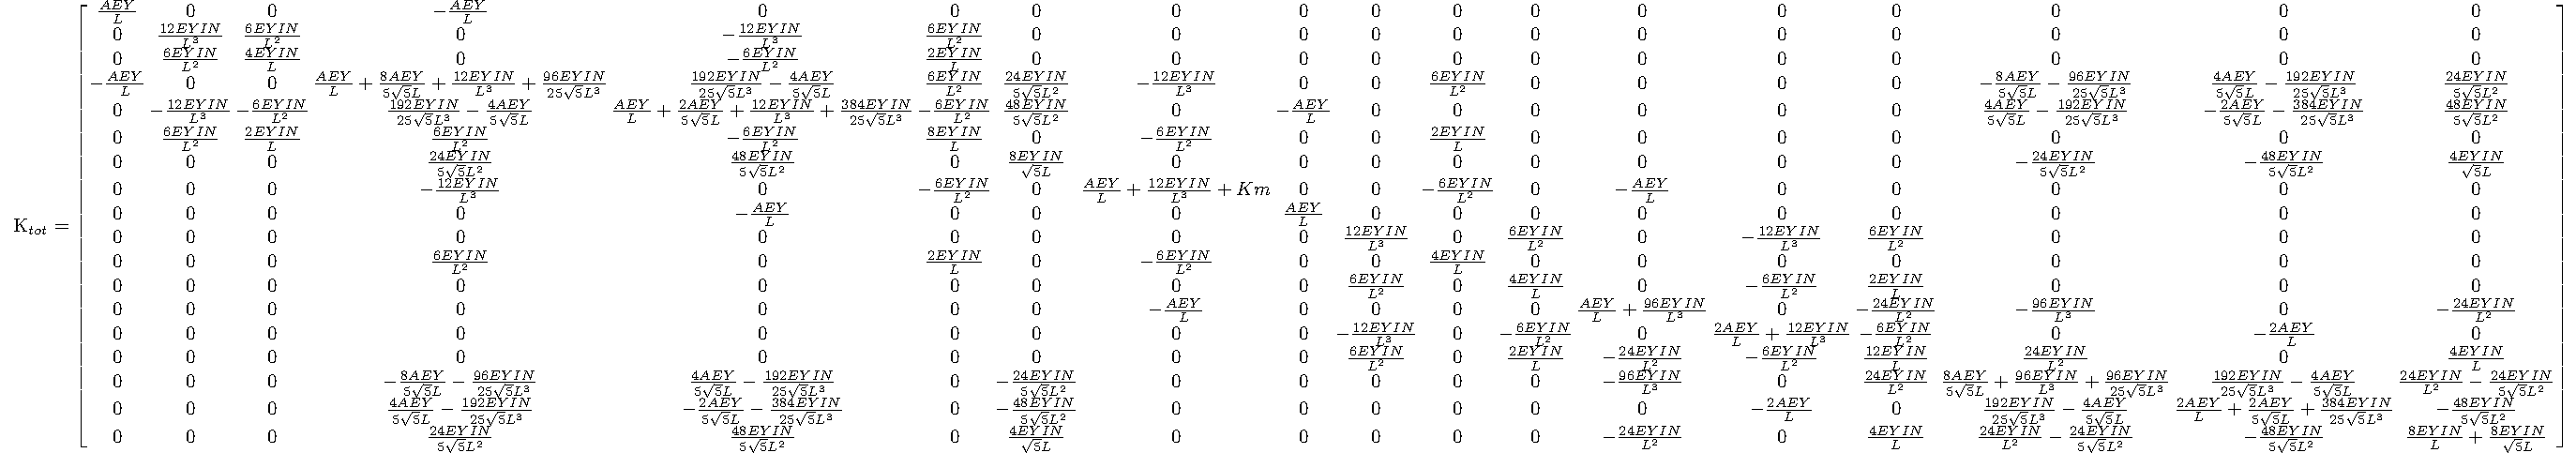
\includegraphics[width=20cm,trim=0 0 23.5cm 0,clip]{rel1/img1/ktot.pdf}}\\  
    
    \vspace{1cm}
    {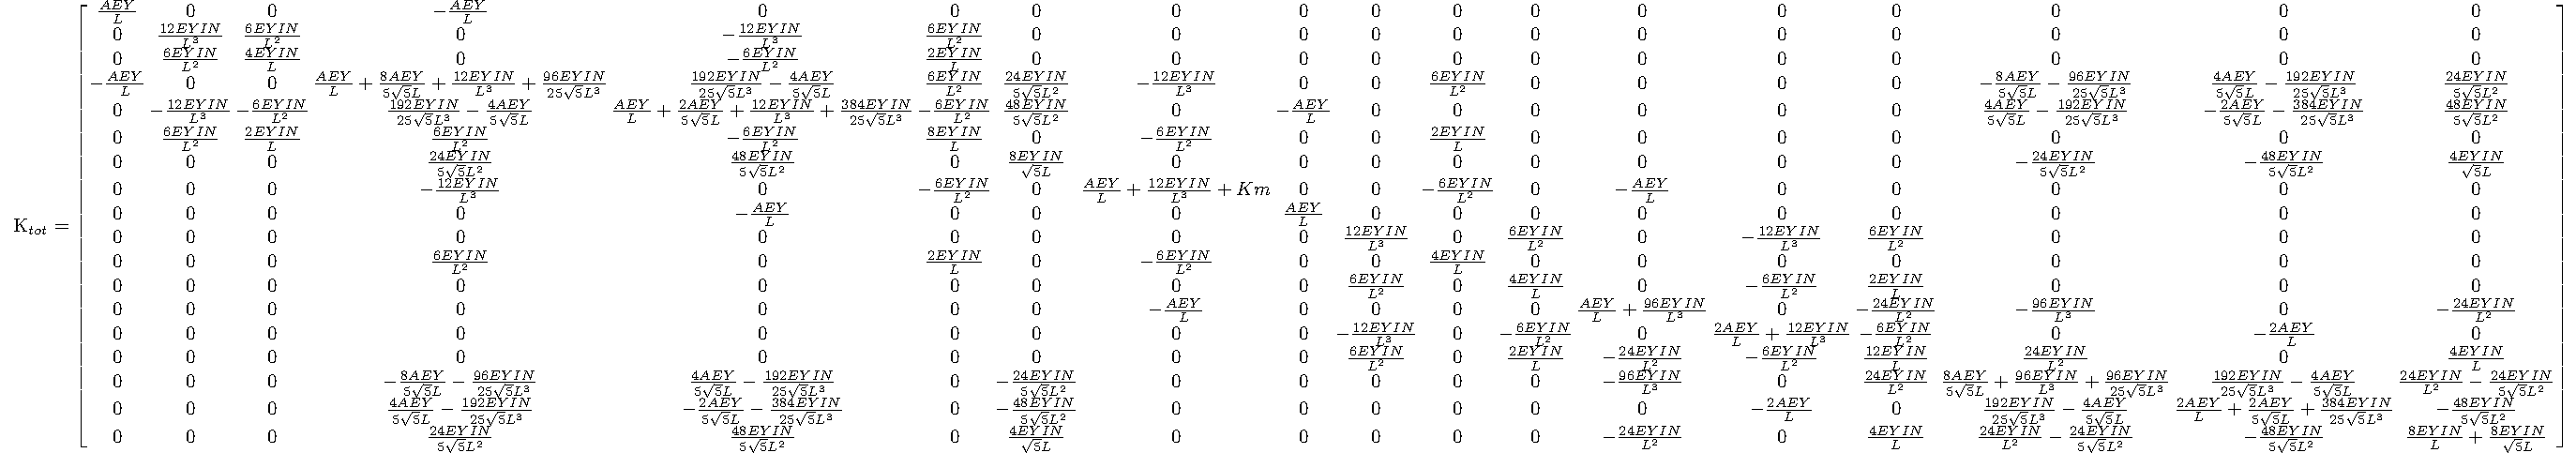
\includegraphics[width=19cm,trim=23cm 0 0 0,clip]{rel1/img1/ktot.pdf}}
    \label{MatriceKtot}
\end{figure}
\end{landscape}
%Risultati U e RV
\[
\label{vet:UeRV}
\overline{u} = \left[
    \begin{array}{c}
    0\\0\\0\\\SI{-7.22e-7}{}\\\SI{6.31e-4}{}\\\SI{3.32e-3}{}\\\SI{8.37e-3}{}\\\SI{4.31e-3}{}\\\SI{6.31e-4}{}\\\SI{3.80e-2}{}\\\SI{3.81e-3}{}\\\SI{-7.35e-3}{}\\\SI{4.32e-3}{}\\\SI{1.76e-2}{}\\\SI{-5.11e-3}{}\\\SI{8.47e-3}{}\\\SI{1.76e-2}{}\\\SI{2.22e-4}{}
    \end{array}
    \right]
\qquad    
\overline{R}_V = \left[
    \begin{array}{c}
    96.07\\\SI{-1.500e3}{}\\\SI{-7.362e3}{}\\0\\0\\0\\0\\0\\0\\0\\0\\0\\0\\0\\0\\0\\0\\0 
    \end{array}
    \right]
\]

    \section{Analisi tramite FEM}
Per la risoluzione con questa metodologia è stato utilizzato il software Abaqus. 
Sono stati scelti degli elementi finiti di tipo $B23$ ovvero elementi alla Eulero-Bernoulli specifici per travi snelle e aventi solamente deformazione assiale e a flessione.

Il nodo $3$ è stato scomposto in due diversi nodi sovrapposti $30$ e $31$, a cui tramite la keyword \lstinline{*EQUATION} è stato imposto che lo spostamento orizzontale nel riferimento globale sia uguale per le due aste.

Si riporta ora l'input utilizzato, mentre nelle tabella \ref{tab:SforziAbaqus} e \ref{tab:SpostamentiUabaqus} sono riportati gli sforzi e gli spostamenti ottenuti.
%Input abaqus
\begin{lstlisting} 
*HEADING
ESERCITAZIONE DI MECCANICA COMPUTAZIONALE
Unita di misura SI (Pa, N, m, ...)
1-asse orizzontale, 2-asse verticale
*PREPRINT, ECHO=YES, MODEL=YES, HISTORY=YES

*NODE, NSET=NALL
10, 0, 0, 0
20, 3, 0, 0
30, 3, 3, 0
31, 3, 3, 0
40, 6, 3, 0
50, 6, 1.5, 0
*ELEMENT, TYPE=B23, ELSET=alfazero
2, 20, 30
3, 31, 40
4, 40, 50
5, 50, 20
*ELEMENT, TYPE=B23, ELSET=alfavero
1, 10, 20
*ELEMENT, TYPE=SPRING1, ELSET=MOLLA
6,30
*SPRING, ELSET=MOLLA
1
22289.6
*RELEASE
5,S2,ALLM
*EQUATION 
2 
30, 1, 1.0, 31, 1, -1.0
*INITIAL CONDITIONS, TYPE=TEMPERATURE
NALL,0
*BEAM GENERAL SECTION, ELSET=alfavero, SECTION=GENERAL
0.0019,0.0000028658,0, 0.0000028658,0
0,0,-1
210000000000,8076923077,0.000012
*BEAM GENERAL SECTION, ELSET=alfazero, SECTION=GENERAL
0.0019,0.0000028658,0, 0.0000028658,0
0,0,-1
210000000000,8076923077,0
*STEP, PERTURBATION
*STATIC
*BOUNDARY
10,ENCASTRE
*CLOAD
50,2,-600
*DLOAD
3,P2,-300
*TEMPERATURE, OP=MOD
10,0,-800,0
20,0,-800,0
*NODE PRINT
U,
RF,
*EL PRINT, POSITION=NODES, SUMMARY=YES
SF,
SM,
*END STEP
\end{lstlisting}
%
\begin{table}[htb]
    \centering
    \caption{sforzi blablsa}
    \label{tab:SforziAbaqus}
    \begin{tabular}{c
                    c
                    S[table-format=-3.3,
                      table-figures-exponent=2,
                      table-sign-mantissa,
                      table-sign-exponent]    
                    S[table-format=-3.3,
                      table-figures-exponent=2,
                      table-sign-mantissa,
                      table-sign-exponent]}
        \toprule
    	\text{Elemento}&\text{Nodo} & \multicolumn{1}{c}{SF1} & \multicolumn{1}{c}{SM1}\\
    	& & \multicolumn{1}{c}{\SI{}{\newton}} & \multicolumn{1}{c}{\SI{}{\newton\meter}}\\
    	\midrule
        1 & 10 & -96.07     & 7.362e3\\
        1 & 20 & -96.07     & 2.862e3\\
        2 & 20 & 0.000       & 2.386e3\\
        2 & 30 & 0.000       & -6.992E-12\\
        3 & 31 & 1.050e3    & -225.0\\
        3 & 40 & 1.050e3    & 1.125e3\\
        4 & 40 & -900.0     & 1.350e3\\
        4 & 50 & -900.0     & 2.925e3\\
        5 & 50 & -1.610e3   & 2.925e3\\
        5 & 20 & -1,610e3   & -5.002E-12\\
        \bottomrule
    \end{tabular}
\end{table}
%Spostamenti
\begin{table}[htb]
    \centering
    \caption{spostamenti abhsajhgsjab}
    \label{tab:SpostamentiUabaqus}
    \begin{tabular}{c
                    S[table-format=1.2,
                      table-figures-exponent=2,
                      table-sign-mantissa,
                      table-sign-exponent]    
                    S[table-format=1.2,
                      table-figures-exponent=2,
                      table-sign-mantissa,
                      table-sign-exponent]
                    S[table-format=1.2,
                      table-figures-exponent=2,
                      table-sign-mantissa,
                      table-sign-exponent]}  
        \toprule
    	\text{Nodo} & \multicolumn{1}{c}{$U_1$} & \multicolumn{1}{c}{$U_2$}& \multicolumn{1}{c}{$UR_3$}\\
    	& \multicolumn{1}{c}{\SI{}{\meter}} & \multicolumn{1}{c}{\SI{}{\meter}}& \multicolumn{1}{c}{\SI{}{\radian}}\\
    	\midrule
        20 & -7.22E-07 & -6.31E-04 & 3.32E-03    \\
        30 & 4.31E-03  & -6.31E-04 & -3.81E-03   \\
        31 & 4.31E-03  & -3.80E-02 & 7.35E-03    \\
        40 & 4.32E-03  & -1.76E-02 & 5.11E-03    \\
        50 & 8.47E-03  & -1.76E-02 & -2.22E-04   \\
        \bottomrule
    \end{tabular}
\end{table}
%-----
\pagebreak
\phantomsection
\section{Confronto spostamenti}\label{cap:cap4}
Come si osserva dalla tabella \ref{tab:SpostamentiUconfronto} a parità di cifre significative, si hanno tutto sommato gli stessi valori per tutti i metodi utilizzati.
\begin{landscape}
\begin{figure}[htb]\centering
\subfloat[][\emph{Momento flettente}]
{
    \begin{tikzpicture}
    \scaling{2.5};
    \begin{scope}[color=lightgray]
        \point{a}{0}{0};
        %\point{b}{.5}{0};
        \point{c}{1}{0};
        \point{d}{2}{.5};
        \point{e}{2}{1};
        \point{f}{1}{1};
        \beam{2}{a}{c}[0][1];
        \beam{2}{c}{d}[1][1];
        \beam{2}{d}{e}[1][1];
        \beam{2}{e}{f}[1][1];
        \beam{2}{f}{c}[1][1];
    \end{scope}
%Diagramma momento:
    \internalforces{a}{c}{.38}{-.6};
    \internalforces{c}{f}{-.6}{0};
    \internalforces{f}{e}{0}{-.3}[-0.1];
    \internalforces{e}{d}{-.3}{-.6};
    \internalforces{d}{c}{-.6}{0};
    \end{tikzpicture}
}
\subfloat[][\emph{Sforzo tagliante}]
{
    \begin{tikzpicture}
    \scaling{2.5};
    \begin{scope}[color=lightgray]
        \point{a}{0}{0};
        %\point{b}{.5}{0};
        \point{c}{1}{0};
        \point{d}{2}{.5};
        \point{e}{2}{1};
        \point{f}{1}{1};
        \beam{2}{a}{c}[0][1];
        \beam{2}{c}{d}[1][1];
        \beam{2}{d}{e}[1][1];
        \beam{2}{e}{f}[1][1];
        \beam{2}{f}{c}[1][1];
    \end{scope}
%Diagramma taglio:
    \internalforces{a}{c}{-.8}{-.8}[0][blue];
    \internalforces{c}{f}{.49}{.49}[0][blue];
    \internalforces{f}{e}{0}{-.45}[0][blue];
    \internalforces{e}{d}{-.55}{-.55}[0][blue];
    \internalforces{d}{c}{.49}{.49}[0][blue];
    \end{tikzpicture}
}
\subfloat[][\emph{Sforzo normale}]
{
    \begin{tikzpicture}
    \scaling{2.5};
    \begin{scope}[color=lightgray]
        \point{a}{0}{0};
        %\point{b}{.5}{0};
        \point{c}{1}{0};
        \point{d}{2}{.5};
        \point{e}{2}{1};
        \point{f}{1}{1};
        \beam{2}{a}{c}[0][1];
        \beam{2}{c}{d}[1][1];
        \beam{2}{d}{e}[1][1];
        \beam{2}{e}{f}[1][1];
        \beam{2}{f}{c}[1][1];
    \end{scope}
%Diagramma normale
    \internalforces{f}{e}{-.32}{-.32}[0][orange];
    \internalforces{e}{d}{.28}{.28}[0][orange];
    \internalforces{d}{c}{.49}{.49}[0][orange]
    \end{tikzpicture}
}
\subfloat[][\emph{Deformazione}]
{
    \begin{tikzpicture}
    \scaling{2.5};
%Indeformata
    \begin{scope}[color=lightgray]
        \point{a}{0}{0};
        %\point{b}{.5}{0};
        \point{c}{1}{0};
        \point{d}{2}{.5};
        \point{e}{2}{1};
        \point{f}{1}{1};
        \beam{2}{a}{c}[0][1];
        \beam{2}{c}{d}[1][1];
        \beam{2}{d}{e}[1][1];
        \beam{2}{e}{f}[1][1];
        \beam{2}{f}{c}[1][1];
    \end{scope}
%Deformata
    \begin{scope}[color=teal]
        \point{n}{1}{-0.01};
        \point{h}{2.03}{.43};
        \point{i}{2.02}{0.93};
        \point{l}{1.01}{.98};
        \point{m}{1.01}{.88} ;
        \beam{2}{a}{n}[0][1];
        \beam{2}{c}{h}[1][1];
        \beam{2}{h}{i}[1][1];
        \beam{2}{i}{m}[1][1];
        \beam{2}{l}{n}[1][1];
    \end{scope}
    \end{tikzpicture}
}    
\caption{Rappresentazione dei diagrammi delle sollecitazioni agenti sulla struttura e la relativa deformata}
\label{fig:DiagrammiFinali}
\end{figure}

\vspace{3cm}
\begin{table}[htb]
    \footnotesize
    \centering
    \caption[Confronto dei risultati degli spostamenti tra i tre diversi metodi utilizzati]{Confronto dei risultati degli spostamenti tra i tre diversi metodi utilizzati. I valori solo da considerarsi riferiti al sistema di riferimento proprio di ciascun metodo}
    \label{tab:SpostamentiUconfronto}
    \begin{tabular}{c
                    S[table-format=1.2,
                      table-figures-exponent=2,
                      table-sign-mantissa,
                      table-sign-exponent]    
                    S[table-format=1.2,
                      table-figures-exponent=2,
                      table-sign-mantissa,
                      table-sign-exponent]
                    S[table-format=1.2,
                      table-figures-exponent=2,
                      table-sign-mantissa,
                      table-sign-exponent]
                      S[table-format=1.2,
                      table-figures-exponent=2,
                      table-sign-mantissa,
                      table-sign-exponent]    
                    S[table-format=1.2,
                      table-figures-exponent=2,
                      table-sign-mantissa,
                      table-sign-exponent]
                    S[table-format=1.2,
                      table-figures-exponent=2,
                      table-sign-mantissa,
                      table-sign-exponent]
                      S[table-format=1.2,
                      table-figures-exponent=2,
                      table-sign-mantissa,
                      table-sign-exponent]    
                    S[table-format=1.2,
                      table-figures-exponent=2,
                      table-sign-mantissa,
                      table-sign-exponent]
                    S[table-format=1.2,
                      table-figures-exponent=2,
                      table-sign-mantissa,
                      table-sign-exponent]}  
        \toprule
        \multirow{3}{*}{Nodo} & \multicolumn{3}{c}{Linea elastica}& \multicolumn{3}{c}{Matriciale}& \multicolumn{3}{c}{Abaqus}\\
    	& \multicolumn{1}{c}{$U_1$} & \multicolumn{1}{c}{$U_2$}& \multicolumn{1}{c}{$UR_3$}& \multicolumn{1}{c}{$U_1$} & \multicolumn{1}{c}{$U_2$}& \multicolumn{1}{c}{$UR_3$}& \multicolumn{1}{c}{$U_1$} & \multicolumn{1}{c}{$U_2$}& \multicolumn{1}{c}{$UR_3$}\\
    	& \multicolumn{1}{c}{\SI{}{\meter}} & \multicolumn{1}{c}{\SI{}{\meter}}& \multicolumn{1}{c}{\SI{}{\radian}}&
    	\multicolumn{1}{c}{\SI{}{\meter}} & \multicolumn{1}{c}{\SI{}{\meter}}& \multicolumn{1}{c}{\SI{}{\radian}}&
    	\multicolumn{1}{c}{\SI{}{\meter}} & \multicolumn{1}{c}{\SI{}{\meter}}& \multicolumn{1}{c}{\SI{}{\radian}}\\
    	\midrule
			2 	&-7.22E-07&6.31E-04&		&-7.22E-07 	&  6.31E-04 & 3.32E-03 	&-7.22E-07 & -6.31E-04 & 3.32E-03 \\
        $3_{sx}$&  &  &  					&4.31E-03  	&  6.31E-04 & 3.80E-03	&4.31E-03  & -6.31E-04 & -3.81E-03\\
        $3_{dx}$&  &  &  					&  			&  3.81E-02 & -7.35E-03	&4.31E-03  & -3.80E-02 & 7.35E-03 \\
       		 4 	&  &  &  					&4.32E-03  	&  1.76E-02 & -5.11E-03	&4.32E-03  & -1.76E-02 & 5.11E-03 \\
       		 5 	&  &  & 					&8.47E-03  	&  1.76E-02 &  2.22E-04	&8.47E-03  & -1.76E-02 & -2.22E-04\\
        \bottomrule
    \end{tabular}
\end{table}
\end{landscape}